\chapter{Design and Implementation}
In this chapter, the design and implementation of a programmable event processing framework within the Open vSwitch are presented. As a preview to the design, the problem statement of the thesis is revisited, and the goals of the implementation are established in section 4.2. The rationale for an Open vSwitch implementation and the overview of the Open vSwitch is presented in sections 4.1 and 4.3. The breakdown of the design and the model of the envisioned system is expressed in section 4.4 and 4.5 respectively. An high-level implementation walk-through is detailed in section 4.6.
Before diving into the design and implementation of the system, it is important to revisit the problem statement and define the goals of the thesis. As outlined in Sections 1.1 and 1.2, the contribution of the thesis is in the area of Event-Based Systems which rely on high streaming data to detect and compose events to be processed. Typically such systems deal with massive streams of data arriving at high rates from a vast variety of nodes - be it sensory nodes or conventional computational devices. In this Chapter, a novel way of offloading the handling of such data onto the underlying network is presented. As outlined in section 1.2, offloading aspects of event processing onto the network can help in reducing the burden of computation on the event processing engines by detecting events and taking appropriate actions before they enter the event processing engine. To create such a solution, the first question that needs to be answered is where in the network can aspects of an event processing engine be offloaded to? The implementation in this thesis focuses on the virtual switch.

With the advent of network and server virtualization environments, virtual switches (vSwitch) have increasingly become the mainstay deployments in all kinds of processing platforms. From large-scale data center networks to smaller Fog deployments, vSwitches allow for communication between different virtualized nodes of a host providing intelligent L2 routing with the aim of abstracting physical switches into an easily manageable logical switch. Since a vSwitch is a pure software solution - embedded or otherwise - it is much easier for administrators to manage and roll-out new functionalities on the switch. Additionally, vSwitches are also deployed on the edge of a network. For these reasons, the implementation in this thesis focuses on offloading aspects of event processing on to a vSwitch. Among the different implementation of vSwitches that are available for researchers today, we focus on the Open vSwitch as the core of our implementation. That leads to the next section, why Open vSwitch? 


\section{Why Open vSwitch?}
Open vSwitch is a production quality switch built for multi-server virtualization environments with highly dynamic nodes. In 2014, an OpenStack survey \cite{OpenStack14} reported that nearly 40\% of production deployments used Open vSwitch, and by 2017 this number had increased to 60\% \cite{OpenStack17}. In addition to large-scale deployments, Open vSwitch has gained popularity in emerging Fog deployments as discussed in sections 3.2 and 3.4. Another key factor in this design is the nature of event processing systems themselves which consist of a rules engine to create new rules based on user logic. Since Open vSwitch supports OpenFlow, a controller can be used to create new event-based rules akin to an event processing system. Figure 4.1 illustrates a take on Open vSwitch performing the role of an event processing engine. Here, a RYU based controller is used to configure event based rules on the Open vSwitch. 
 \begin{figure}[H]
 \centering
 \caption{Open vSwitch viewed as an Event Processing engine} 
 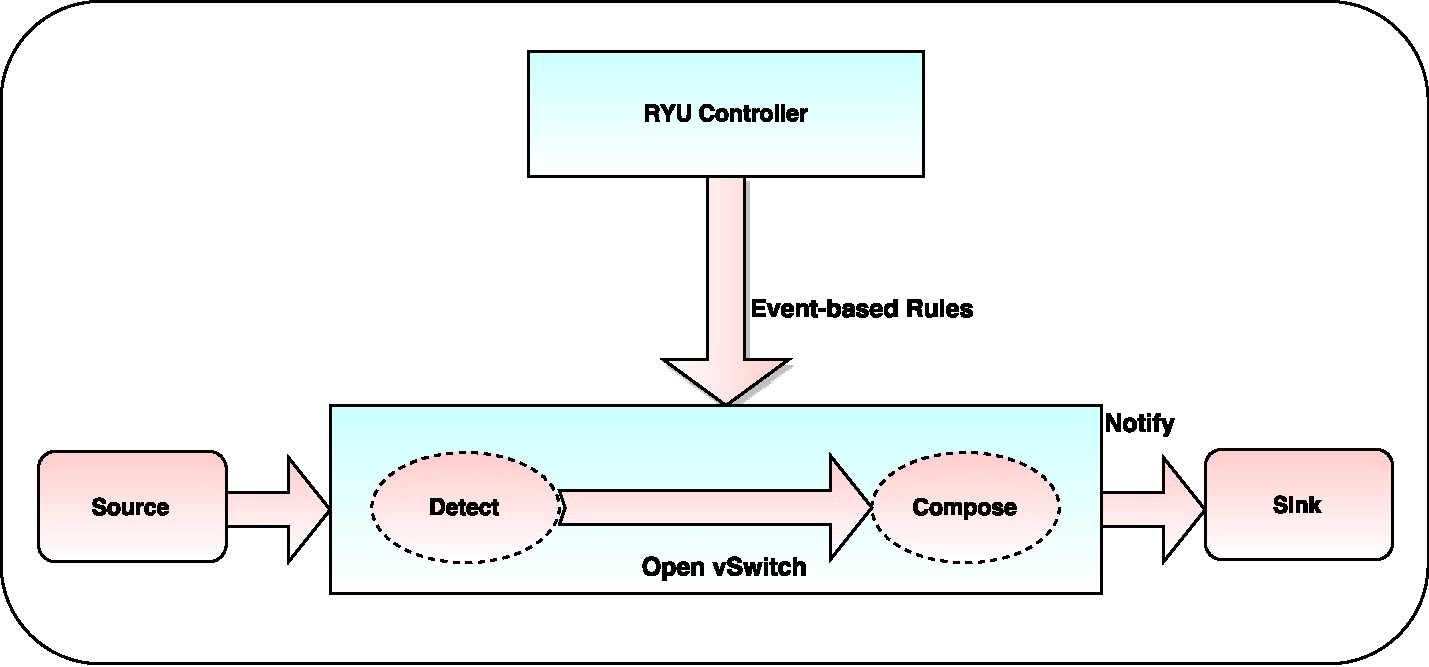
\includegraphics[height=8cm,width=14cm]{evsep01.pdf}
\end{figure}

\section{Goals of the implementation}
Goals of the implementation are defined as below:
\begin{itemize}
\item An Open vSwitch implementation is provided to detect event types and steer them to facilitate staged processing without having to context switch into an intermediate computing node.
\item The Open vSwitch implementation focuses on the DPDK datapath to take advantage of the accelerated packet I/O offered by the DPDK libraries.
\item The Open vSwitch is enabled to execute simple logical operations on the data items of an event and filter based on application logic. 
\item A Ryu controller-based implementation is provided to enable applications to offload user logic on to the vSwitch using an HTTP and JSON based northbound API.
\end{itemize}
Having defined the goals of the thesis, it is important to understand the internals of the Open vSwitch and examine design decisions that need to be taken to achieve the goals outlined.

\section{An overview of Open vSwitch}
In this section a brief overview of the three most important components in the Open vSwitch \cite{pfaff2015design}
\begin{itemize}
 \item \textbf{ovs-vswitchd}: ovs-vswitchd is the generic userspace daemon which speaks OpenFlow and controls all the switches in a system. The ovs-vswitchd daemon is responsible for the OpenFlow pipeline for packet processing and also determines how a packet has to be handled for the first time before it is cached in the datapath. The ovs-vswitchd daemon instructs the datapath on how to handle the packet depending on the configurable OpenFlow processing pipeline. The daemon communicates with the Open vSwitch kernel module via the Netlink interface, and with the ovsdb-server using the custom ovsdb management protocol.
 \item \textbf{ovsdb-server}: The ovsdb-server provides the runtime for the lightweight ovsdb database that holds switch-level configurations. On reboot, the switch configurations are persisted in the ovsdb and are applied when the daemon comes back up. Currently, ovsdb supports state information in the form of 13 different tables for bridges, ports, interfaces, flow tables, controllers, etc. among others.
 \item \textbf{Kernel Datapath}: The kernel datapath or the kernel module is the host operating system implementation of an exact match cache. It is unaware of OpenFlow or the state of the switch. It is kept simple for highly performant packet lookup and forwarding. The ovs-vswitchd receives the first packet from the datapath module, looks up the packet in the OpenFlow processing pipeline, gathers the actions and caches it in the kernel datapath. The following packets of the same flow are forwarded using the caches entries in the datapath without having to go to the userspace daemon(upcall).
\end{itemize}

In addition to the three components is the OpenFlow controller. The controller keeps the state of the network and can be installed on the same server or a remote server. The controller speaks OpenFlow with the ovs-vswitchd daemon and can be used to remotely configure the OpenFlow processing pipeline of several remote switches. The controller may also be used to persist flow of the ovs-vswitchd daemon in the case of a crash. The overview of these components is shown in figure 4.2 - sourced and reinterpreted from \cite{pfaff2015design}.
In addition to the above components, the implementation provides several management utilities:
\begin{itemize}
 \item \textit{ovs-vsctl}: This utility is used to configure the ovsdb-server with several switch configurations such as adding or deleting bridges, adding/deleting ports, etc. The utility connects directly to the ovsdb-server -
 \item \textit{ovs-ofctl}: This utility is used to monitor and configure the OpenFlow switches. It connects directly to the ovs-vswitchd daemon via OpenFlow and provides commands to add new flow rules to the OpenFlow pipelines among several other commands to monitor the flow statistics for the switches and ports.
 \item \textit{ovs-dpctl}: This utility connects to the ovs-vswitchd daemon and provides commands to monitor the cached datapath flows. It offers several commands such as add/delete flows to/from the datapath, monitor statistics, etc. among several others.
 \item \textit{ovs-appctl}: This utility is a used for runtime configuration of the ovs-vswitchd daemon, such as configuring logging levels of the different modules within Open vSwitch.
 \item \textit{ovsdb-tool}: This utility is used to manage the ovsdb files. It offers commands to create DB schemas and compact existing schemas. It does not interact with the ovsdb-server.
 \item \textit{ovsdb-client}: This utility offers a command-line interface to interact with the running ovsdb-server using the different JSON-RPC methods specified by ovsdb management protocol. It offers commands to run transactions such as insert, delete into the ovsdb, dump tables, monitor columns, etc. among others.
\end{itemize}

In the context of the thesis, most of the work focuses on the ovs-vswitchd daemon and the OpenFlow processing pipeline. In the following section the internal flow of data once a packet hits the physical device is presented.

 \begin{figure}[H] 
  \centering   
 \caption{OVS components}
 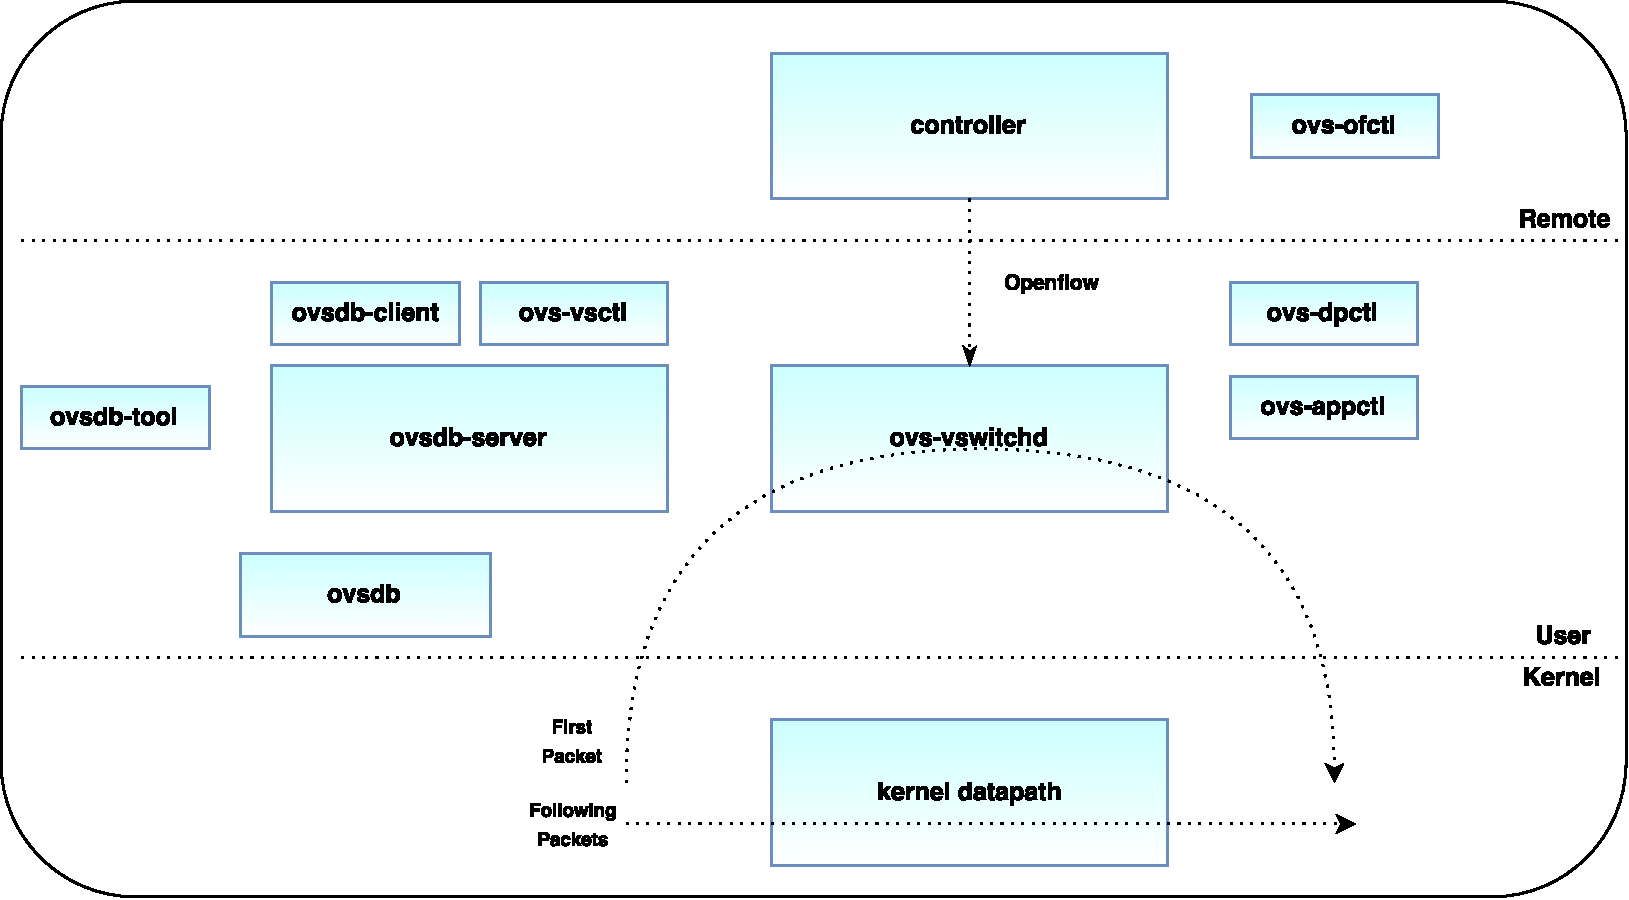
\includegraphics[height=10cm]{kernaldatapath.pdf}
\end{figure}

The interplay of the components of the Open vSwitch is shown in figure 4.3. The two interfaces that specify the handling of the packets are \newline
\textbf{Datapath interface}: The datapath in the context of Open vSwitch is a flow cache capable of forwarding packets through a port. The datapath of an Open vSwitch is implemented specifically to the host machine, and it relies on its clients for intelligence. In this case, the intelligence for the datapath is provided by the ovs-vswitchd. The generic datapath interface provided by Open vSwitch is dpif. The userspace implementation of the datapath interface is provided by the \textit{dpif-netdev} module. The dpif provides an interface with abstractions for three key components:
\begin{itemize}
 \item Ports: Each datapath has a set of ports akin to Ethernet ports. In case of the dpdk or userspace datapaths, the implementation for these ports comes from \textit{struct netdev}, with \textit{netdev-dpdk} specifically handling dpdk ports.
 \item Flow table: A flow table has three key entities: flow - which consists of L2, L3, and L4 headers. The datapath flow uses the \textit{struct dpif-flow}; mask - corresponding to each bit in a flow. The mask field is used for the megaflows, and not for the exact match cache; actions - which tell the datapath what to do with the packet.
 \item Upcalls: The datapath notifies the clients, which is the ovs-vswitchd in this case, about a flow table miss or userspace actions using upcalls. During the upcall, the whole packet is copied to the userspace using the struct \textit{dp_packet}.
\end{itemize}

 \begin{figure}[H] 
 \centering   
 \caption{OVS overview}
 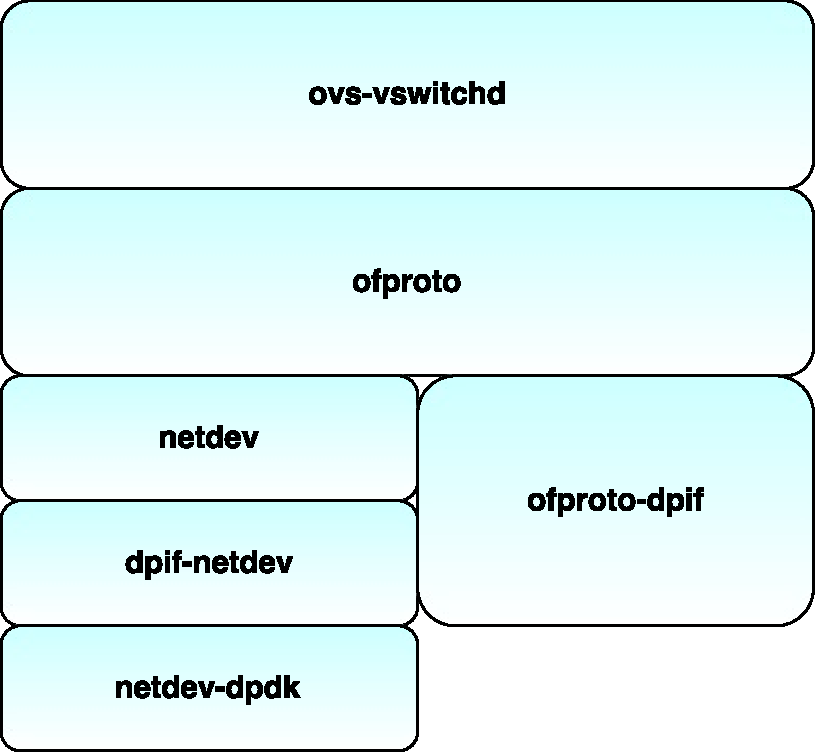
\includegraphics[height=6cm]{internals.pdf}
\end{figure}

\textbf{Ofproto Interface}: The ofproto interface implements the OpenFlow protocol implementation for the dpif-netdev interface. It consists of three major components:
\begin{itemize}
 \item oproto-dpif: This module implements the main provider of the OpenFlow abstraction. It is responsible for installing and removing datapath flows, monitoring and maintaining statistics, etc. The ofproto.dpif module also is responsible for deciding whether a flow is to be cached or not.
 \item ofproto-dpif-upcall: This module performs the role of retrieving the upcalls from the datapath. It performs simple processing of missed upcalls and interacts with ofproto-dpif for complex processing.
 \item ofproto-dpif-xlate: This module performs the role of looking up the OpenFlow processing pipeline, extracting OpenFlow actions and translating into datapath actions.
\end{itemize}

\section{Design Breakdown}
Before design and implementation of the event processing framework within Open vSwitch, a brief breakdown of the design and rationale is provided. The design details are presented in the later sections. Key aspects that require our focus are:
\begin{itemize}
 \item Extraction of events from the payload: While work done by  Mekky et. al \cite{mekky2014application} concentrates on creating OpenFlow actions to direct packets into a separate application module to work on the payload, the work in this thesis focuses on extracting the payload at line rate. The rationale behind this approach is that event queries are applied on each packet in the system, and directing the packets to a separate application module is expensive when the same action has to be repeated for every single packet.
 \item De-serializing the event payload: The data items in the event stream are encoded. In the thesis, a solution is provided for de-serializing hexadecimal encoded streams of data. 
 \item Accessing the event data: Once the event items are extracted and encoded from the event stream, they must be made accessible for processing within the Open vSwitch and also be accessible by OpenFlow rules that are installed on the controller. Due to this reason, the design focuses on modifying the OpenFlow 1.0 protocol spoken between the controller and the Open vSwitch. Although OpenFlow 1.3 is the most standard protocol in use, the work in the thesis uses OpenFlow 1.0 for simplicity. Porting from OpenFlow 1.0 to 1.3 is not considered to be a blocking factor.
 \begin{figure}[H] 
 \centering   
 \caption{OVS dataflow: datapath to ofproto}
 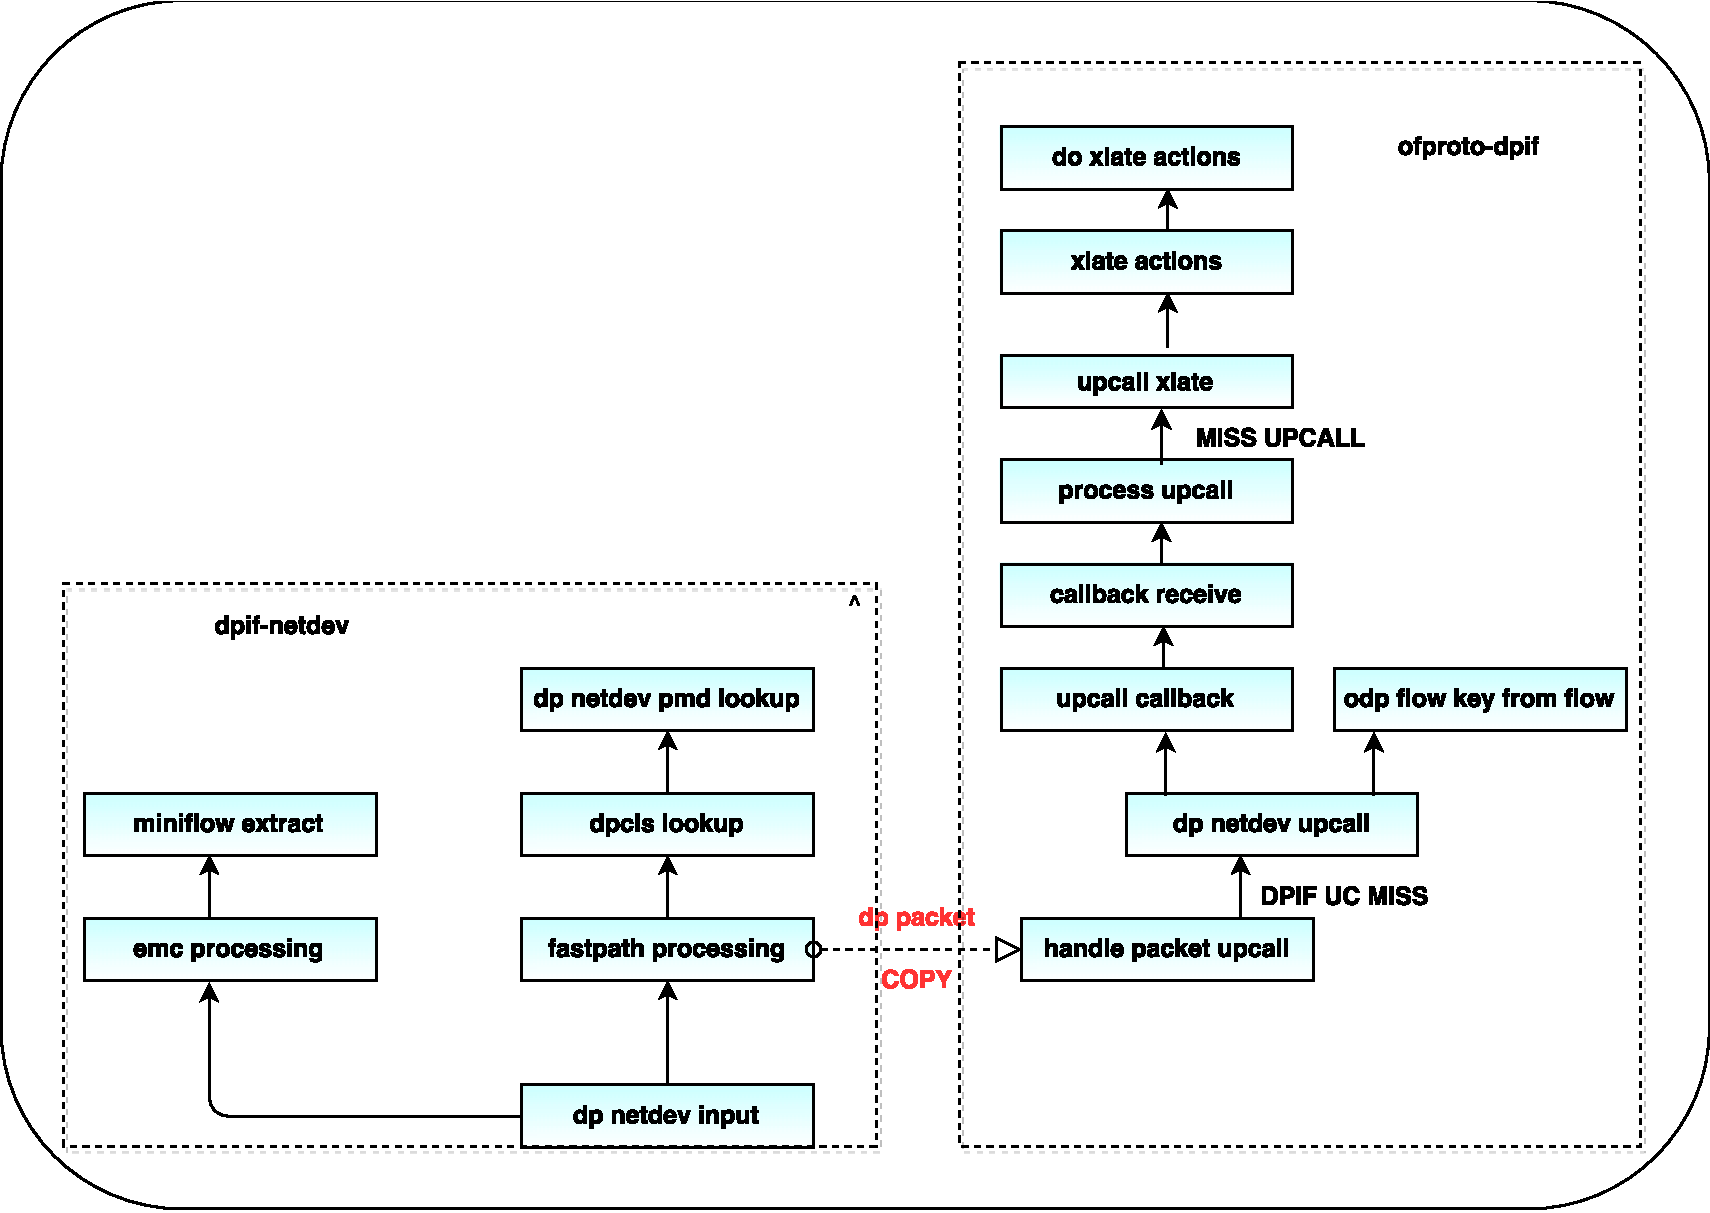
\includegraphics[height=12cm]{dpnetdev.pdf}
\end{figure}
 \item OpenFlow pipeline support for events: For making the event detection programmable, additional tables are created within the OpenFlow processing pipeline, or the ofproto classifier. Handling the ofproto classifier is sufficient because ofproto-dpif takes care of creating the tables in the datapath classifier/exact match cache when needed.
 \item Creating keys for event attributes: The \textit{odp-netlink} interface in Open vSwitch specifies the rules for creating attribute keys. These keys are used to look up the ofproto classifier and find the relevant rule installed for an event. 
 \item Support for logical operations: The operations on event attributes are performed using OpenFlow actions. Hence each operation is achieved using a newly defined action, which is triggered based on the detection criteria specified on event items.
 \item RYU Controller design: The controller plays a big role in communicating OpenFlow rules to the Open vSwitch. Although ovs-ofctl utility can also play this part, a controller such as RYU is more sophisticated, in that it allows the creation of HTTP API's that are accessible by remote webservers to create rules. Such an API support is provided which enables remote creation and deletion of event based rules. The RYU controller plays the role of the rules engine, whereas Open vSwitch plays the role of the execution engine. 
\end{itemize}

The design overview presented above aims to create a sophisticated programmable event processing framework on the network, which can complement the event processing engines to achieve latency sensitive results, reduce the burden of computation and enable staged processing. In the coming sections, more focus is granted up on individual design decisions.


\section{System Model}
In this sections, the supported semantics for event processing within the Open vSwitch is presented. Each event follows the below representation:\\1. Unique Tag\\
2. Event Type\\3. Event Attributes


To this end the event payload format processed by the framework within Open vSwitch is pre-defined. Each event has a unique tag,  followed by the event type and two event attributes. Only the packets with the unique tag are processed through the event processing pipeline. In other cases, the packets are taken through the standard processing pipeline within Open vSwitch. The event payload handled by the event processing engine is shown in figure 4.5. The timestamp in the event is used for evaluation purposes.

\begin{figure}[H]
 \centering
 \caption{Event Payload}
 \includegraphics[width=10cm]{payload.pdf}
\end{figure}

\subsection{Event Detection Semantics}
Let 'E' be an event of type 't' and attributes '$a_1$' and '$a_2$'.

\begin{equation}
E\lbrace t,a_1,a_2 \rbrace
\end{equation}

The event detection semantic understood and processed by the framework are described below:

\begin{flushleft}
 Event instances can be detected based on different variants.
 \\1. Detect based on Event Type
 \\2. Detect based on values in Event Attributes
 \\3. Detect based on combination of Event Type
 \\
\end{flushleft}
\begin{flushleft}
 Event detection operations can be combined with logical operators:
 \\
 \textbf{Conjunction}: Event is signalled when all constituent input patterns evaluate to True. 
 \\
 \textbf{Disjunction}: Event is signalled when atleast one constituent input pattern evaluates to True.
 \\

\end{flushleft}


\begin{flushleft}
The detect operations that are implemented are denoted as:

\begin{equation}
D(e.t) \quad | \quad stream
\end{equation}
\begin{equation}
D(e.t) \quad | \quad filter
\end{equation}
\begin{equation}
D(e.t  \wedge e.a_1) \quad | \quad stream
\end{equation}
\begin{equation}
D(e.t  \wedge e.a_1) \quad | \quad filter
\end{equation}
\begin{equation}
D(e.t  \wedge e.a_2) \quad | \quad stream
\end{equation}
\begin{equation}
D(e.t  \wedge e.a_2) \quad | \quad filter
\end{equation}
\begin{equation}
D(e.t  \wedge (e.a_1 \wedge e.a_2)) \quad | \quad stream
\end{equation}
\begin{equation}
D(e.t  \wedge (e.a_1 \wedge e.a_2)) \quad | \quad filter
\end{equation}
\begin{equation} 
D(e.t  \wedge (e.a_1  \vee e.a_2 )) \quad | \quad stream
\end{equation}
\begin{equation} 
D(e.t  \wedge (e.a_1  \vee e.a_2 )) \quad | \quad filter
\end{equation}

where \textit{D} is the detect operation; \newline
| denotes the redirect operation; \newline
\textit{stream} is the logical stream to which the detected event is redirected to.\newline
\textit{filter} is the operation to filter the detected event \newline \newline
\end{flushleft}


\subsection{Compare Operation Semantics}
In addition to event detection based on match of event attributes, compare operations on event attributes are implemented. The set of implemented compare operators is given by:
\begin{equation}
\oplus  \ni  \lbrace <=,>= \rbrace
\end{equation}

and the possible operations using the compare operators is given by:
\begin{equation}
D(e.t  \wedge (e.a_1 \oplus value) \vee e.a_2) \quad | \quad filter
\end{equation}
\begin{equation}
D(e.t  \wedge (e.a_1 \oplus e.a_2) \quad | \quad filter
\end{equation}
\subsection{Stateful Operation Semantics}
Stateful operations in the context of the implementation are defined as those that use the knowledge of previous events to take an action on the currently detected event. The two stateful operations implemented are moving maxima and window.

\begin{equation}
D(e.t  \wedge (e.a_1  <=\quad \rightarrow maxvalue) ) \quad | \quad filter
\end{equation}
In this operation all the events with attribute lower than the given \textit{maxvalue} are filtered. However, on the detection of an event with a value higher than the given \textit{maxvalue}, the event is forwarded and the newly seen value becomes \textit{maxvalue}.
\begin{equation}
D(e.t  \wedge (e.a_1  <=\quad \overrightarrow{win} \quad maxvalue)) \quad | \quad filter
\end{equation}
Similar to 4.15,  all the events with attribute lower than the given \textit{maxvalue} are filtered. However, on the detection of an event with a value higher than the given \textit{maxvalue}, the event is forwarded and the newly seen value becomes \textit{maxvalue}. The \textit{maxval} increases for a window of \textit{win} events after which it remains steady. if the window is 0, this is equivalent to less than or equal to operation defined in 4.14.

\section{Implementation walk-through}
In this section, the key aspects of implementing a programmable event processing framework within an Open vSwitch are discussed. The implementation aims to meet the specifications defined in the system model in section 4.5 and follows the design strategy discussed in section 4.4. Wherever appropriate the implementation is discussed along with data or control flow diagrams, snippets of code or data structures used in the implementation.

\subsection{Event extraction and de-serialization}
In this section, the methodology for event parsing and extraction is presented. Before chalking up a strategy, the flow of data in the DPDK/userspace datapath is examined more closely in figure 4.4. As it can be seen in the figure, the packet is handed over to the ofproto interface in its entirety using the data structure \textit{dp_packet}. But if the event data is extracted only after passing it to ofproto, this would mean that any support of the exact match cache or the datapath classifier that can be provided by the DPDK datapath to the event processing extension is ruled out. Hence the parsing and extraction of the event payload is done within the dpif-netdev implementation using the flow module. Once the event is extracted, it is de-serialized. Both the steps are done within the flow module of the Open vSwitch. 

\begin{figure}[H]
 \centering
 \caption{Event extraction and access}
 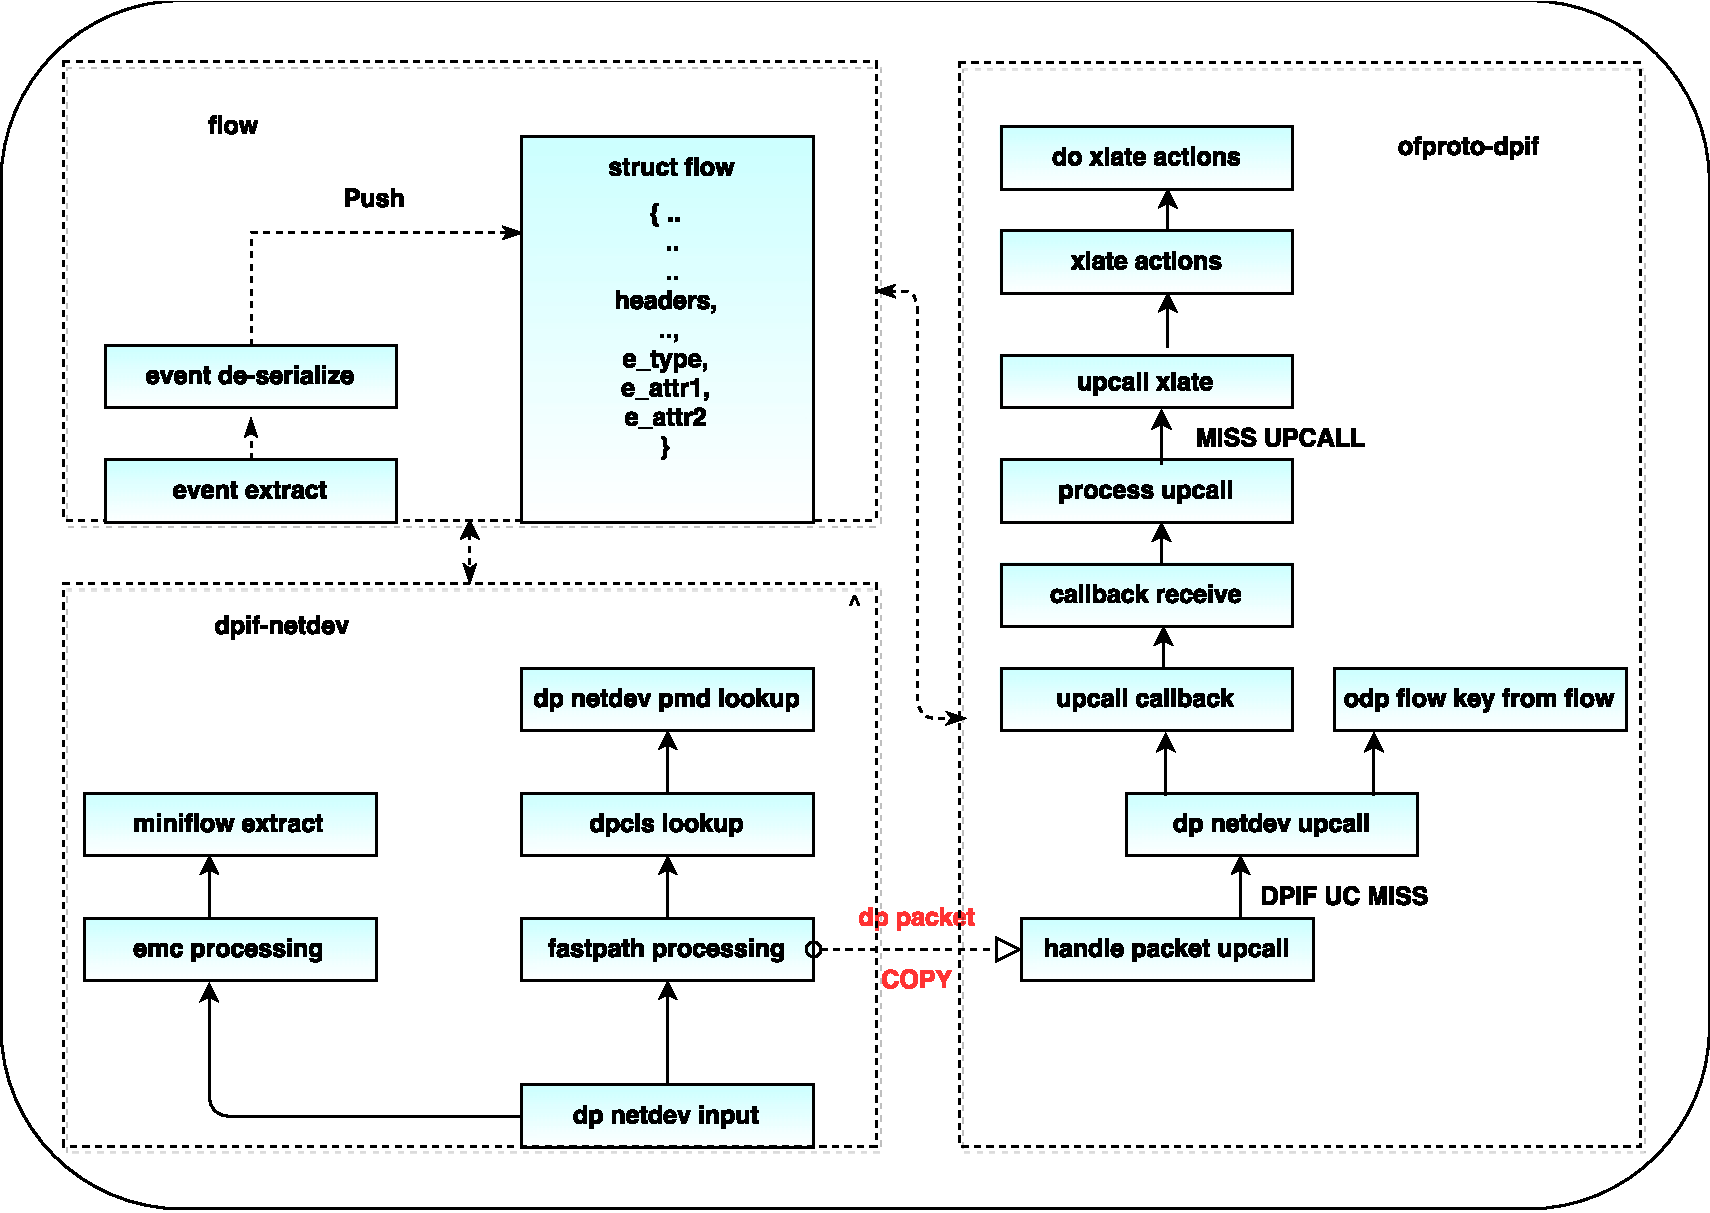
\includegraphics[height=12cm]{flowextract01.pdf}
\end{figure}

\subsection{Accessing event data}
Once the data items are extracted and de-serialized, they are being made accessible to the implementations of both the ofproto interface and datapath interface. The flow module of the Open vSwitch specifies the data structures for the OpenFlow fields, which are accessible by both the userspace dpif-netdev and ofproto implementation. Additionally, since the extraction and de-serialization of the event data is performed within the flow module, the support for event data items is added into the userspace flow data structure \textit{struct flow}. Doing so ensures that the event data is accessible to the ofproto and the datapath interface, and also to the yet to be discussed meta-flow module which specifies the interface for the Open vSwitch implementation of OpenFlow 1.0 tables. Figure 4.6 shows the interplay of the modules while extracting, de-serializing and pushing the data to the relevant data structure for access within other modules. The flow module also provides another data structure \textit{struct flow_wildcards} which follows the same structure as flow, except that each 1-bit in wildcard indicates that the corresponding bit in \textit{struct flow} must match. For the event data items, only an exact match is supported. Hence all the bits of the struct \textit{flow_wildcards} for event data items are set. Below snippet shows the addition of support for event data in struct flow and the map used to access the flow by other interfaces. \newline

\begin{lstlisting}[language=c]
struct flow {
..
..
..
/* L4 (64-bit aligned) */
ovs_be64 e_type;
ovs_be64 e_attr1;
ovs_be64 e_attr2;
..
..
}

FLOWMAP_SET(map, e_type);  
FLOWMAP_SET(map, e_attr1);  
FLOWMAP_SET(map, e_attr2);  


miniflow_push_be64(mf, e_type, htonll(event[0]));                   
miniflow_push_be64(mf, e_attr1, htonll(event[1]));
miniflow_push_be64(mf, e_attr2, htonll(event[2]));
\end{lstlisting}



\begin{figure}[H]
 \centering
 \caption{Openflow Pipeline}
 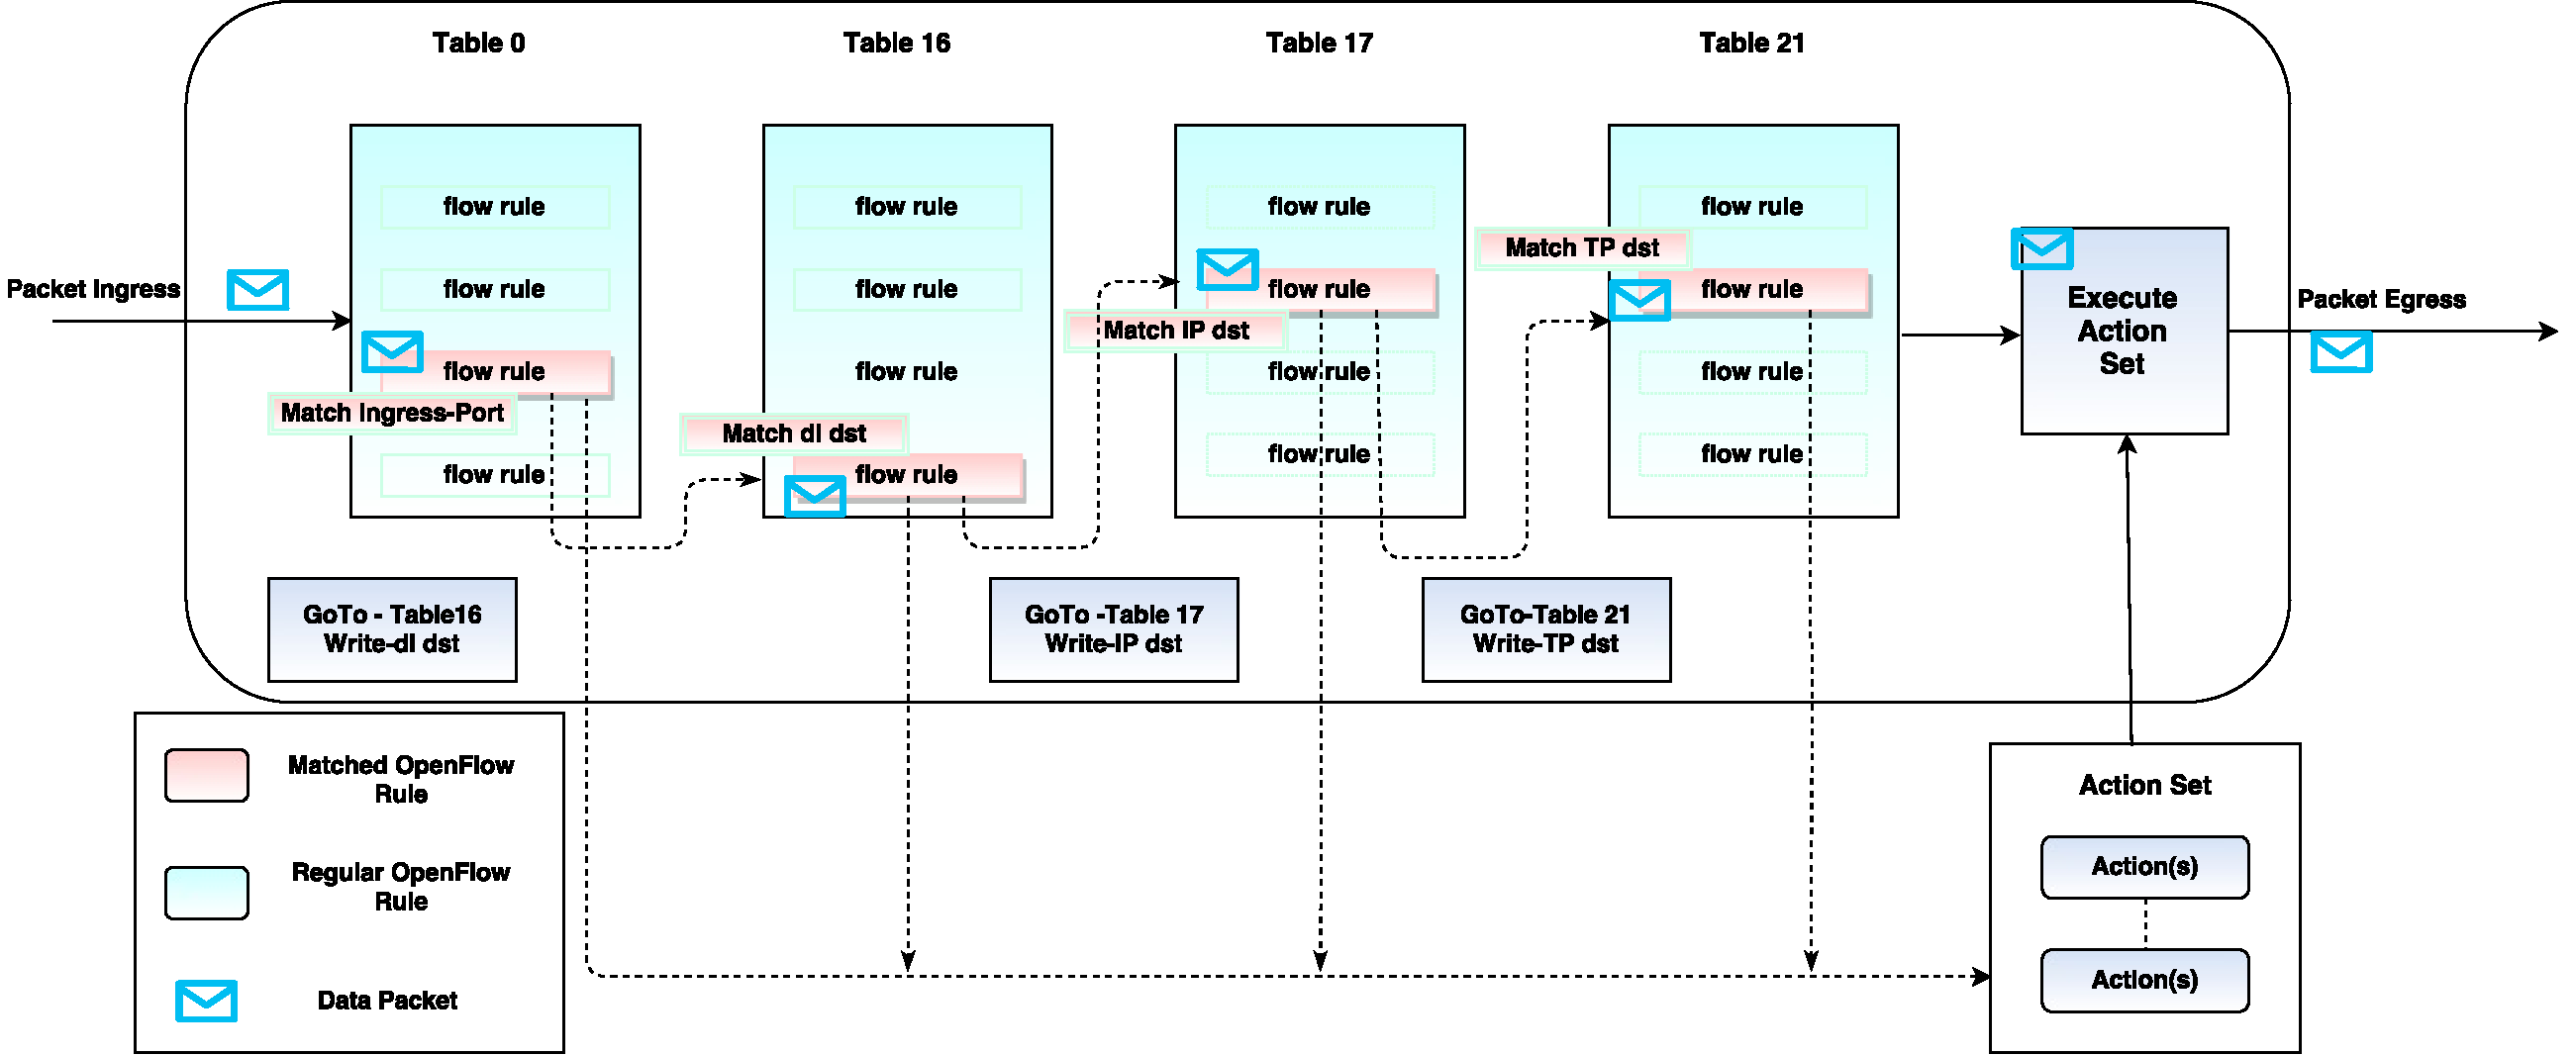
\includegraphics[height=8cm,width=19cm]{pipeline05.pdf}
\end{figure}

\subsection{Modelling OpenFlow pipeline for event processing}
As briefly alluded to in the section 4.6.2, the event items are to be added into the OpenFlow processing pipeline. The specification of OpenFlow 1.0 protocol is available within Open vSwitch in the Openflow-1.0 modules. The meta-flow module defines the interface to implement the OpenFlow processing pipeline, i.e., the fields of the ofproto classifier. Before diving into the implementation details, we examine the ofproto classifier pipeline in figure 4.7. OpenFlow supports pipelined processing of packets with the help of multiple tables which in turn have multiple flow rule entries. In figure 4.7, the incoming packet at the ingress port is matched at Table 0, the action of rewriting the mac destination address is added to the action-set and submitted to Table 16. At Table 16, the packet is matched on its mac destination address, and the action of re-writing its IP destination address is added to action-set is performed, and it is forwarded to Table 17. At Table 17, the packet is matched by a flow rule for its IP destination address, and the action of re-writing its Transport destination address is added to the action-set, and the packet is forwarded to Table 21. At Table 21 the packet is matched by a flow rule for its Transport destination address and checked for GO-TO instruction in rule action. Since no GO-TO instruction is found, the pipeline processing stops and the action-set is executed on the packet, and the packet is forwarded through the egress port. For the sake of simplicity, the focus in this thesis document will be on a single OpenFlow table. Although enabling one OpenFlow table to handle event data is sufficient to create an OpenFlow pipeline for event data, such a use case is not helpful initially. Figure 4.8 shows an individual flow table and the steps taken to enable event fields within it. 

\begin{figure}[H]
 \centering
 \caption{Openflow Flowtable - Add event data fields}
 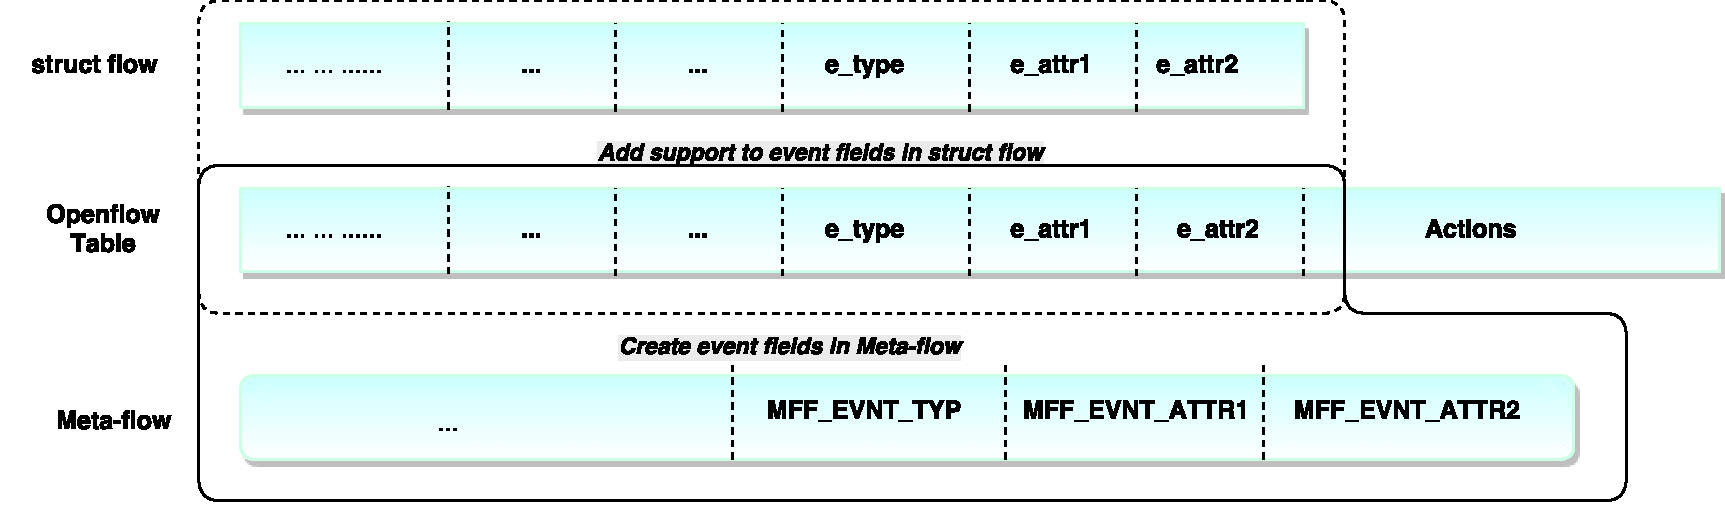
\includegraphics[height=5cm]{flowtable.pdf}
\end{figure}

\subsection{Adding event data fields to OpenFlow tables}
 As discussed in section 4.6.2 the data structure flow is modified to handle event data and provide access to the event data to the ofproto interface. Predictably, similar support is to be added to the OpenFlow table using the meta-flow module as shown in figure 4.8. Below is the snippet which shows the creation of the event type as an OpenFlow field within the meta-flow module. \newline

\begin{lstlisting}
/* "e_type".
*
* Event Type.
*
* Type: be64.
* Maskable: bitwise.
* Formatting: decimal.
* Prerequisites: UDP.
* Access: read/write.
* NXM: NXM_OF_EVNT_TYP(113) since v2.6.
* OXM: OXM_OF_EVNT_TYP(46) since OF1.2 and v2.6.
* OF1.0: exact match.
* OF1.1: exact match.
*/    
MFF_EVNT_TYP,
\end{lstlisting}


The comments for the meta-flow field are expected to be in the exact format specified for the python helper function extract-ofp-fields. Failing to do so results in build breakdown. In addition to adding fields in the meta-flow module, the fields are provided with necessary helper functions which are accessed by ofproto and ofp-parse interfaces while responding to flow-mod or flow stats request commands from the controller. One such helper function defined to set e_type from the corresponding met-flow field is shown below. This function is used to read the meta-flow field and populate match before dumping the buffer for dump-flow commands. Similarly, other helpers are defined. \newline
\begin{lstlisting}[language=c]
void
mf_set_value(const struct mf_field *mf,
const union mf_value *value, struct match *match, char **err_str)`{
 ..
 ..
 case MFF_EVNT_TYP:
 match_set_event_type(match, value->be64,OVS_BE64_MAX);
 break; 
 ..
 ..
 
}
\end{lstlisting}

\subsection{Adding support for event based rules}
Adding event fields in the meta-flow module enables support for event data in the OpenFlow table. It, however, is not sufficient to enable event-based rules and detection of events based on extracted data. This is done in two stages
\begin{itemize}
\item Provide support to event fields in add-flow command of ovs-ofctl utility to send the relevant data in OpenFlow message. This command is also used by the controller. More about the controller implementation is discussed later.
\item Add support to decode event fields from the incoming OpenFlow message and insert the event based rules into the classifier.
\end{itemize}
Before diving into the details, the important interfaces are examined:
\begin{itemize}
\item \textbf{ofp-parse interface}: The ofp-parse interface specifies the layer of communication between ovs-vswitchd and OpenFlow. In the case of the flow-mod commands(OFPC_ADD), ofp-parse module converts the string value pairs of the event fields and inserts them into the match field of data structure \textit{struct ofp_util_flow_mod}.
\item \textbf{ofp-util interface}: The ofp-util interface defines the the \textit{struct ofp_util_flow_mod} to consume and respond to the flow-mod commands. The struct \textit{struct ofp_util_flow_mod} is composed of a struct match as a member. 
\item \textbf{match interface} The match interface provides the data structure for flow classification - \textit{struct match}. Each match structure consists of a flow and a corresponding wildcard.  The ofp-parse and ofp-util interface combine to extract the string-value pairs in a flow-mod command into relevant flows and wildcards within a \textit{struct match}. 
In addition to creating event based flow rules, functionality is also implemented to dump event based flow rules on to the buffer as in case of dump-flows command. For this operation, within the match module, helper functions to get meta-flow event fields into the \textit{struct match} are also defined. This is used by the ofp-parse interface to populate \textit{struct match} and hand it over to nx-match interface for encoding. An example of such an helper function is shown in the below snippet: \newline
\begin{lstlisting}[language=c]
void
match_set_event_type_masked(struct match *match, ovs_be64 e_type, ovs_be64 mask){
match->flow.e_type = e_type & mask;
match->wc.masks.e_type = mask;
}
\end{lstlisting}

\item \textbf{nx-match module}: The flow and the wildcards from the match interface are encoded as fields defined by the meta-flow module using the nicira extension helper functions specified by the nx-match module. Doing so enables dump-flow support to event-based rules.
\end{itemize}

Figure 4.9 shows how a OFPFC_ADD command with event fields is parsed and normalized into the match interface using \textit{struct ofputil_flow_mod}. To enable correct parsing of the event fields, OpenFlow 1.0 support is configured in Openflow-1.0 header file: \newline

\begin{lstlisting}[language=c]
enum ofp10_flow_wildcards {
..
OFPFW10_EVNT_ATTR1 = 1 << 22,
OFPFW10_EVNT_ATTR2 = 1 << 23,
OFPFW10_EVNT_TYP   = 1 << 24,
..
}
\end{lstlisting}
This informs the parser that the relevant event fields are in the 22, 23 and 24 positions of the character string. After which the relevant event fields are populated and normalized. Normalization ensures that the corresponding wildcards for the match flow entries are appropriately set. Once normalized the flow-mod command is encoded as a OFPT_FLOW_MOD message and send to the ovs-vswitchd daemon which actively polls for OpenFlow messages.

\begin{figure}[H]
 \centering
 \caption{Openflow: Parse event fields}
 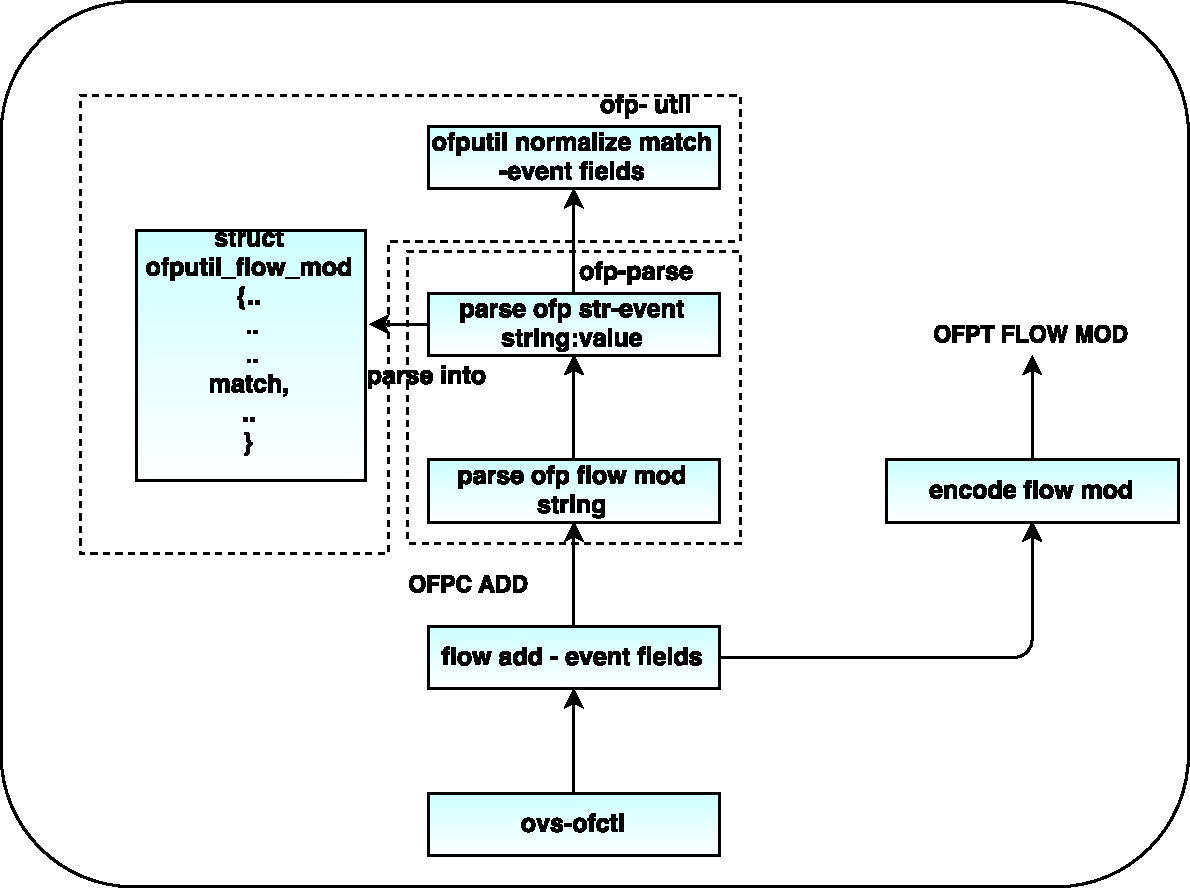
\includegraphics[height=10cm,width=14cm]{flowadd.pdf}
\end{figure}

Figure 4.10 shows an OpenFlow message of type OFPTYPE_FLOW_MOD is parsed to extract the relevant rules and added into the classifier. The ovs-vswitchd daemon actively polls for OpenFlow messages. On receiving a message, the message type is decoded. If the message is of type 'OFPTYPE_FLOW_MOD' the message is decoded by a decode function. The first phase of the decoding process involved pulling the message which is in the custom OpenFlow buffer, ofpbuf, into the Openflow1.0 match structure struct ofp10_match. This structure is also extended to support event fields, very much like struct flow: \newline

\begin{lstlisting}[language=c]
struct ofp10_match {
..
ovs_be64 e_attr1;
ovs_be64 e_attr2;
ovs_be64 e_type;
}
\end{lstlisting}

Once the \textit{struct op10_match} is created, the relevant event fields are extracted and put into a \textit{struct match} and normalized. The ofpbuf is not directly pulled into \textit{struct match} because the match interface is inaccessible outside the context of ovs-vswitchd. Instead, the ofp-util interface is used to convert the data OpenFlow structures to a form understandable and accessible by the OpenFlow implementation within Open vSwitch, i.e., ofproto. Once the rules are stored in the form of a match, the ovs-vswitchd daemon calls the ofproto interface to add the rules into the classifier.

\begin{figure}[H]
 \centering
 \caption{Openflow: Event rule creation}
 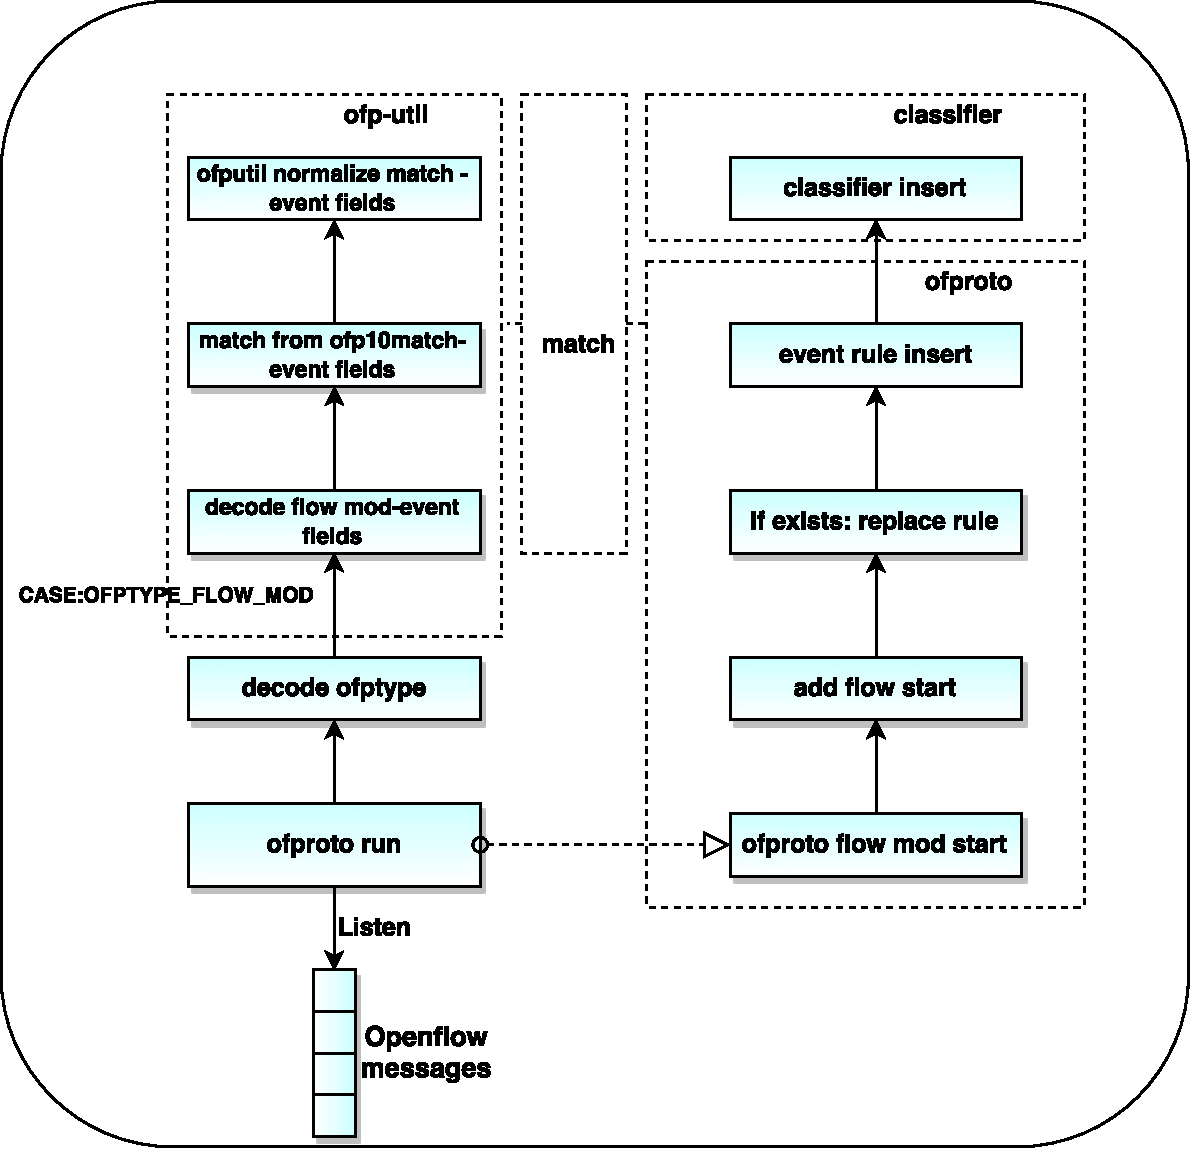
\includegraphics[height=12cm,width=14cm]{ruleinsert.pdf}
\end{figure}

At this point, the implementation supports programmable event rules and the three event fields specified by the system model. However, the event detection mechanism is yet to be implemented. In the next subsection, a closer look into the implementation steps needed to support matching based on event type and event attributes is presented.

\subsection{Detection based on event data}
In this section, the implementation process to support classifier lookup based on event fields. In section 4.6.2, event data is pushed into the flow structure, and in section 4.6.3 to 4.6.5, event rule support is added to the OpenFlow processing tables- i.e., ofproto classifier. To look up the classifier with the event data items, event keys are extracted from the flow. Figure 4.11 illustrates the lookup process followed by the ofproto-dpif-xlate module.

\begin{figure}[H]
 \centering
 \caption{ofproto: Rule look-up}
 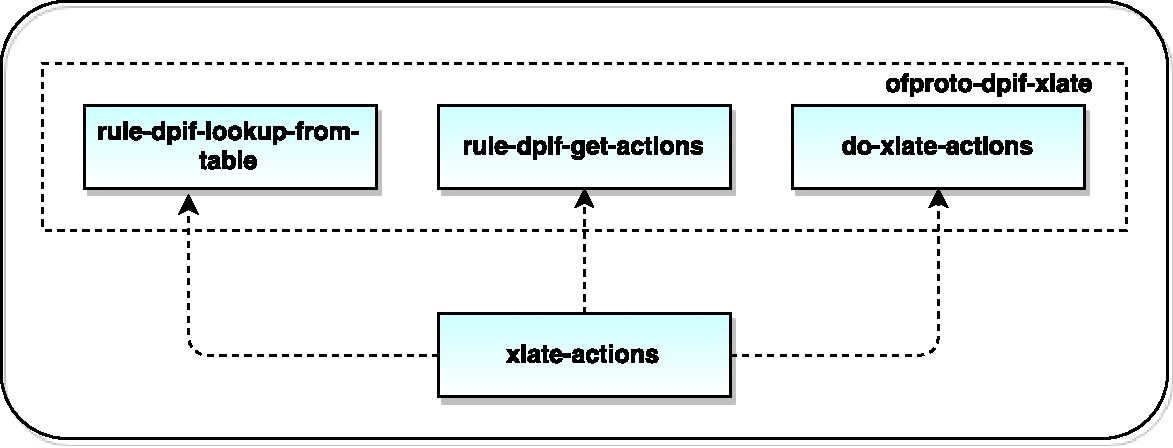
\includegraphics[height=5cm]{ofproto-dpif-xlate.pdf}
\end{figure}

Userspace keys to support the lookup are added to odp-netlink. In the below snippets, the set up steps for \textit{e_type} key are shown. The snippet focuses on the key steps to be taken to enable keys and excludes the details, which can be found in the source code. \newline

\begin{lstlisting}[language=c]
enum ovs_key_attr {
..
#ifndef __KERNEL__
/* Only used within userspace datapath*/ 

OVS_KEY_ATTR_EVNT_TYP,
#endif
..
};

struct ovs_key_etype {
ovs_be64 e_type;
};

\end{lstlisting}

and the keys are parsed and extracted to be used by ofproto-dpif. \newline
\begin{lstlisting}[language=c]
/* parse_l2_5_onward */
if (!is_mask) {
..
..
 expected_attrs |= UINT64_C(1) << OVS_KEY_ATTR_EVNT_TYP;
}

if (present_attrs & (UINT64_C(1) << OVS_KEY_ATTR_EVNT_TYP)) {
 const struct ovs_key_etype *etype_key; 
 etype_key = nl_attr_get(attrs[OVS_KEY_ATTR_EVNT_TYP]);
 put_etype_key(etype_key, flow);
}

/* odp_flow_key_from_flow  and odp_flow_key_from_mask*/
 struct ovs_key_etype *etype_key;  
etype_key = nl_msg_put_unspec_uninit(buf, OVS_KEY_ATTR_EVNT_TYP,
sizeof *etype_key); 
\end{lstlisting}

At this stage, the implementation supports event rules that implement operations denoted through 4.2 to 4.11, by combining existing event semantics with drop and mod actions provided by OpenFlow. In Section 5.4.7, many of these operations are evaluated with their respective rule format supported by the RYU controller. The operations are also contrasted with their expression in a standard Event Query language.



\subsection{Enabling compare operations support}
As discussed in section 4.2, the thesis also aims to provide support for logical operations on event attributes. In section 4.5.2 the two compare operators {>=, <=} are outlined for implementation. In this section the implementation of the compare operations within Open vSwitch is presented. The operations are implemented as Openflow actions which are triggered after detecting a event type. The two compare operations are implemented as:
\begin{itemize}
 \item \textbf{set_max} : A \textit{set_max:val} action ensures that any event with attribute value higher than \textit{val} is filtered out for a particular event type.
 \item \textbf{set_min} : A \textit{set_min:val} action ensures that any event with attribute value lower than \textit{val} is filtered out for a particular event type.
\end{itemize}
The \textit{set_max}, \textit{set_min} actions provide implementation support for operations denoted in 4.13. The implentation can be extended for any binary operaiton The code snippets illustrate  how the new actions are added to the Openflow action list, with \textit{set_max} action used for illustration. \newline

\begin{lstlisting}[language=c]

OFPACT(SET_MAX,ofpact_attr, ofpact, "set_max")      
/* OFPACT_SET_MAX.
*
* Used for OFPAT10_SET_MAX.*/
struct ofpact_attr {
 struct ofpact ofpact;
 uint64_t attr;              /* Attribute value. */
};
\end{lstlisting}

In addition implementation support is provided to parse, decode, encode and set attributes for actions. The implemetnation for the user actions is done in the ofproto-dpif-xlate module which as discussed before and illustrated in figure 4.11 is responsible for deriving actions and performing them. \newline
\begin{lstlisting}[language=c]
case OFPACT_SET_MAX:{        
 if(htonll(flow->e_attr1) <= ofpact_get_SET_MAX(a)->attr){
  xlate_normal(ctx);
 }
 break;    
}
\end{lstlisting}

In addition to comparing attributes to values provided in event rules; another class of action is implemented which allow creation of rules to compare between the attributes themselves. This is done via:
\begin{itemize}
 \item \textbf{attr_cmp}: A \textit{attr_cmp:mode} action compares the event attributes, and filters out the events based on the mode triggered by \textit{val}. if \textit{mode} is 0, only events with equal attributes is forwarded, rest are dropped. if \textit{mode} is 1, only events with attribute 1 greater than attribute 2 are forwarded, if \textit{mode} is 2, only events with attribute 2 greater than attribute 1 are forwarded. Here \textit{mode} triggers the operation to be used between attributes. Similarly implementations can be extended for any other binary operation.
\end{itemize}
The  \textit{attr_cmp} action provides the implementation of operations denoted in 4.14.

\subsection{Enabling Stateful Operations}
In this section the implementation of stateful operations denoted in section 4.5.3 is detailed. To implement these operations two actions are implemented:
\begin{itemize}
 \item \textbf{mov_max}: A \textit{mov_max:maxval} action filters the event if the attribute is lower than \textit{maxval}. However if the attribute value higher than \textit{val} is encountered, the event is forwarded and the newly seen value becomes the new \textit{maxval}. This action provides implementation support to the operation denoted in 4.15. Below the pseudo-code of the \textit{mov_max} action is shown:\newline
 \begin{lstlisting}[language=c]
 case OFPACT_SET_MOV_MAX: 
 mov_max= ofpact_get_SET_MOV_MAX(a)->attr
 item= search_max(type)
 if(item!=NULL):                         
  cur_max = item->data
  if(attr1 > cur_max):
   delete_max(item)
   insert_max(type, attr1)                
 else:
  cur_max = mov_max
  insert_max(type, mov_max)
 if(attr1 < cur_max):
   break
 else:  
  xlate_normal(ctx)  
  break  
 \end{lstlisting}
 
 \item \textbf{set_win,win_max}: The combination of \textit{set_win:win,win_max:maxval} actions performs a similar role done by the \textit{mov_max}. However the \textit{maxval} is incremented only for the specified window \textit{win}, after which it remains constant. To understand this action, let us look at an example for event type 'TEMP', with action \textit{set_win:10,win_max:50}. Firstly all events of type 'TEMP' with attribute values lower than 50 are filtered. An event of type 'TEMP' and attribute value 60 is forwarded, and 60 becomes the new \textit{maxval}. And going forward, a 'TEMP' event with value 58 will be filtered. This increment of \textit{maxval} continues till the 10th window, or otherwise the 10th time the rule is hit. From thereon, the highest value of attribute seen within the defined window will remain the \textit{maxval}. This action provides implementation support to the operation denoted in 4.16. The below pseudo-code glimpses through the implementation.
 
\begin{lstlisting}[language=c]
case OFPACT_SET_WIN:
window= ofpact_get_SET_WIN(a)->attr
winItem=search_window(type)
if(winItem == NULL):
 insert_window(type, window, 0)                       
else:
 delete_window(winItem)
 insert_window(type, window, ++(winItem->counter))       
break;

case OFPACT_SET_WIN_MAX:
mov_max= ofpact_get_SET_WIN_MAX(a)->attr 
winItem=search_window(type)
item= search_max(type)
if(>window <= counter):
 if(item!=NULL):
  cur_max = item->data 
 else
  cur_max = mov_max
else if(window > counter):
 if(item!=NULL):                     
  cur_max = item->data
  if(attr1 > cur_max):
   delete_max(item)
   insert_max(type, htonll(flow->e_attr1))                     
 else:
  cur_max = mov_max
  insert_max(type, mov_max)
if(attr1 < cur_max): 
 break
else:
 xlate_normal(ctx);   
 break
\end{lstlisting} 
\end{itemize}

\subsection{API support for event rules via RYU}
In this section, the implementation of an OpenFlow based event rules engine is presented. To implement support for event rules the RYU controller is modified. Figure 4.12 shows the flow of data within the RYU controller started from the API to the corresponding \textit{OFPT_FLOW_MOD} message. 

\begin{figure}[H]
 \centering
 \caption{RYU: North to South - Event Rule creation}
 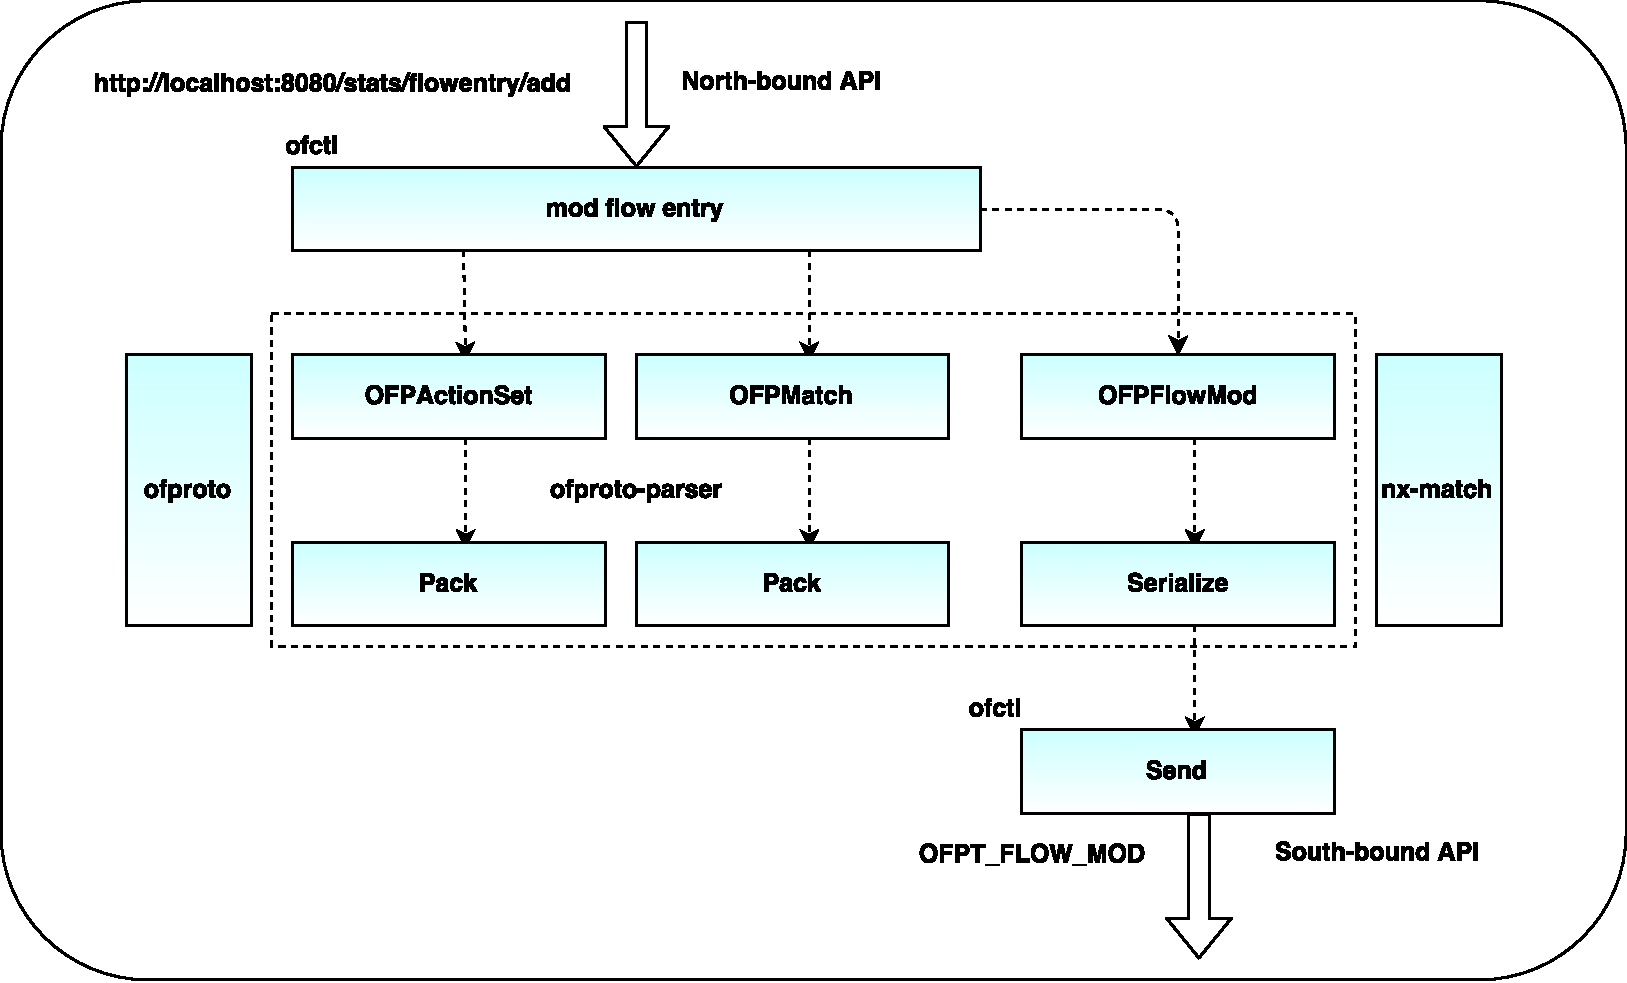
\includegraphics[height=10cm,width=14cm]{ryu01.pdf}
\end{figure}
The implementation is broken down into four parts:
\begin{itemize}
 \item \textbf{ofproto}: In the ofproto module all the event related fields are initialized, and their positions in the OpenFlow message is set. The position set in this module mirror the Open vSwitch support for the event fields. In addition to this, the ofproto module also defines the packing structure the flow-mod message sent to Open vSwitch. In the below snippet, the mapping of event fields and actions between the controller and Open vSwitch is shown. \newline
 
 \begin{lstlisting}[language=python]
 _OFP_MATCH_PACK_STR = 'IH' + OFP_ETH_ALEN_STR + 's' + OFP_ETH_ALEN_STR + \
 'sHBxHBB2xIIHHQQQQ' 
 
 OFPAT_SET_WIN_MAX = 12  # window moving max value for attribute1.
 OFPAT_SET_MOV_MAX = 13  # moving max value for attribute1.
 OFPAT_SET_MIN = 14      # min value for attribute1.
 OFPAT_SET_MAX = 15      # moving max value for attribute1.
 OFPAT_SET_WIN = 16      # window value
 OFPAT_SET_CMP = 17      # compare mode
 
 OFPFW_EVNT_ATTR1 = 1 << 22
 OFPFW_EVNT_ATTR2 = 1 << 23
 OFPFW_EVNT_TYP = 1 << 24
 \end{lstlisting}
 
 \begin{lstlisting}[language=c]
 struct ofpact_map of10[] = {
 ..
 { OFPACT_SET_WIN_MAX, 12},
 { OFPACT_SET_MOV_MAX, 13},
 { OFPACT_SET_MIN, 14},
 { OFPACT_SET_MAX, 15},
 { OFPACT_SET_WIN, 16},
 { OFPACT_SET_CMP, 17}
 ..
 }
 enum ofp10_flow_wildcards {
 ..
 OFPFW10_EVNT_ATTR1 = 1 << 22,
 OFPFW10_EVNT_ATTR2 = 1 << 23,
 OFPFW10_EVNT_TYP   = 1 << 24,
 } 
 \end{lstlisting}
 \item \textbf{nx-match}: In the nx-match module, the methods to serialize the match structure is defined with methods to put each event fields and the respective wild cards into the defined header fields This module takes care of the serialization of the match fields and their wildcards. In the below snippet, the serialization process is show for the event type field. \newline
 
 \begin{lstlisting}[language=python]

 @_register_make
 @_set_nxm_headers([ofproto_v1_0.NXM_OF_EVNT_TYP])
 class MFEVNTTYP(MFField):
 @classmethod
 def make(cls, header):
 LOG.debug('VLOG in point 76')
 return cls(header, MF_PACK_STRING_BE16)
 
 def put(self, buf, offset, rule):
 LOG.debug('VLOG in point 86')
 return self.putm(buf, offset, rule.flow.e_type, rule.wc.e_type_mask)
 
 def serialize_nxm_match(rule, buf, offset):
 if rule.flow.e_type != 0:
 if rule.flow.nw_proto == 17 and rule.wc.e_type_mask == UINT64_MAX:
 header = ofproto_v1_0.NXM_OF_EVNT_TYP
 else:
 header = 0
 if header != 0: 
 offset += nxm_put(buf, offset, header, rule)
 \end{lstlisting}

 \item \textbf{ofctl}: The ofctl module consists of the implementation for the \textit{mod_flow_entry} method which handles the north-bound HTTP enabled flowadd API. In this module, the event fields and actions are extracted from the JSON messages, reads them to previously defined match fields which are sent to the ofproto parser module to pack them into the desired format. \newline
 \begin{lstlisting}
 #read from JSON into e_type string:value pair
  match = dp.ofproto_parser.OFPMatch(wildcards,.. e_type,..) #call OFPMatch
 
 #read from json into set_max string:value pair
 elif action_type == 'SET_MAX':
 val = int(a.get('val', 0))
 actions.append(dp.ofproto_parser.OFPActionSetMax(val))  #call OFPActionSet
 \end{lstlisting}

 \item \textbf{ofproto-parser}: The ofproto-parser module is modified to taking the match and action strings containing event related messages and convert them into Flow and Action structures supporting the relevant event fields and actions. The ofproto-parser module packs relevant structures using the definition provided in the ofproto module and then serializes the message using the methods provided in nx-match modules. The message sent out to the Open vSwitch is a \textit{OFPT_FLOW_MOD} message which is defined in position 14 within the Open vSwitch and hence is packed similarly in RYU. \newline
  \begin{lstlisting}[language=python]
  OFPT_FLOW_MOD = 14       # Controller/switch message
     \end{lstlisting}
     
     In Open vSwitch:
     \begin{lstlisting}[language=c]
  enum ofpraw { 
  /* OFPT 1.0 (14): struct ofp10_flow_mod, uint8_t[8][]. */
  OFPRAW_OFPT10_FLOW_MOD}
  \end{lstlisting}
  
  The below snippet shows the methods added to parse and serialize individual event \textit{set_min} action. \newline 
  
 \begin{lstlisting}[language=python]
 class OFPActionAttrVal(OFPAction):
 def __init__(self, val):
  super(OFPActionAttrVal, self).__init__()
  self.val = val

 @classmethod
 def parser(cls, buf, offset):
  type_, len_, val = struct.unpack_from(
  ofproto.OFP_ACTION_ATTR_VAL_STR, buf, offset)
  assert type_ in (..,
  ofproto.OFPAT_SET_MIN,
  ..)
  assert len_ == ofproto.OFP_ACTION_ATTR_VAL_SIZE
  return cls(val)
 
 def serialize(self, buf, offset):
  msg_pack_into(ofproto.OFP_ACTION_ATTR_VAL_STR,
  buf, offset, self.type, self.len, self.val) 
 
 
 @OFPAction.register_action_type(ofproto.OFPAT_SET_MIN,
 ofproto.OFP_ACTION_ATTR_VAL_SIZE) 
 \end{lstlisting} 

\end{itemize}

\subsubsection{Enable Northbound API}
In addition to changes in the different modules, the Northbound API support is provided to the RYU application by mapping the /flowentry/add command to the mod_flow_entry method within ofctl. The format of the JSON and the usage to add event-based rules into the Open vSwitch is discussed in detail along with examples in the next chapter. \newline


\begin{lstlisting}[language=python]
uri = path + '/flowentry/{cmd}'
mapper.connect('stats', uri,
controller=StatsController, action='mod_flow_entry',
conditions=dict(method=['POST']))
\end{lstlisting}


\section{Summary}
In this chapter, the design and implementation of a programmable event processing framework within Open vSwitch with the RYU controller used as the rules engine was presented. The chapter characterized the goal of the thesis, presented a design breakdown and depicted a system model for events. Three classes of event semantics were expressed within the system model after which the steps taken to implement the system was recounted with necessary illustrations of data flow and snippets of code necessary for fair representation. In the next chapter, the evaluation of the system across several parameters is chronicled with a brief discussion of relevant results.

